%!TEX root = edance.tex
\graphicspath{{./figs_semi/}}


\chapter{Introduction to Semiconductors}




\subsection{Chapter Preview}

In this chapter we'll build models for conductors and semiconductors, starting with the simplest model of all, an ideal metal with a "gas" of electrons swarming about and study conduction in this ideal system.  Surprisingly, we'll find that many properties of real conductors are captured with this model.  Next, we'll delve into semiconductors and learn why the model breaks down.  We'll briefly look a the structure of semiconductors and then develop a simple bond model that can account for free carriers, especially when a material is "doped", or when impurities are added to a solid to modulate its conductivity.  With this model in hand, we'll discuss drift and diffusion currents.  Drift currents are already familiar conduction of electrons in response to a field, or Ohm's Law, whereas diffusion current is due to concentration gradients, which play an important role in devices like diodes.  




\section{Conduction in an Ideal Metal ``Gas''}


\subsection{Ohm’s Law}

 One of the first things we learn in electrical engineering and physics is that  $V = I \times R$.
 Is this trivial? Maybe what’s really going on is the following:
\begin{equation}
	V = f(I) = f(0) + f'(0)I + f''(0){I^2}/2 + ... \approx f'(0)I
\end{equation}
 In the above Taylor expansion, if the voltage is zero for zero current, and the current is small, then this is generally valid for a reasonably smooth function.   The range of validity (radius of convergence) is the important question. It turns out to be VERY large!
 
\subsection{Ohm’s Law Revisited}
  
In Physics we learned:  $J = \sigma \,E$  Is this also trivial? Well, it’s the same as Ohm’s law, so the questions are related. For a rectangular solid:
\begin{equation}
	J = \frac{I}{A} = \sigma \,\frac{V}{L} \end{equation}\begin{equation}  V = \frac{L}{{\sigma \,A}}I = R\,I
\end{equation}
Isn’t it strange that current (velocity) is proportional to Force?  Where does conductivity come from?

 
\subsection{Conductivity of a Gas}

 Electrical conduction is due to the motion of positive and negative charges.   For example, for  water with pH=7, the concentration of hydrogen H+ ions (and OH-) is:

\begin{equation}
{10^{ - 7}}{\rm{mole/L}} = {\rm{1}}{{\rm{0}}^{{\rm{ - 10}}}}{\rm{mole/c}}{{\rm{m}}^{\rm{3}}} 
= {\rm{1}}{{\rm{0}}^{{\rm{ - 10}}}} \times 6.02 \times {10^{23}}{\rm{c}}{{\rm{m}}^{ - 3}} 
= 6 \times {10^{13}}{\rm{c}}{{\rm{m}}^{ - 3}}
\end{equation}
Typically, the concentration of charged carriers is much smaller than the concentration of neutral molecules.   The motion of the charged carriers (electrons, ions, molecules) gives rise to electrical conduction.
 

\subsubsection{Collisions in Gas}

At a temperate $T$, each charged carrier will move in a random direction and velocity until it encounters a neutral molecule or another charged carrier.  Since the concentration of charged carriers is much less than molecules, it will most likely encounter a molecule. For a gas, the molecules are widely separated ($\sim 10$ molecular diameters).  After colliding with the molecule, there is some energy exchange and the charge carrier will come out with a new velocity and new direction.
 
\subsubsection{Memory Loss in Collisions}
  
Schematically our model thus far is shown in Fig.~\ref{fig:slide8}.   The key point is the initial velocity and direction is lost (randomized) after a few collisions.


\begin{figure}
\begin{center}
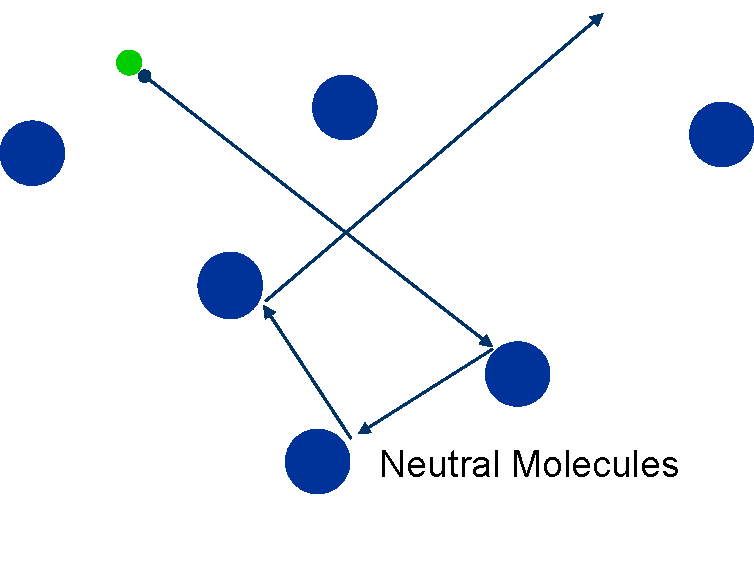
\includegraphics[width=.5\columnwidth]{slide8}
\end{center}
\caption{X. } \label{fig:slide8}
\end{figure}
 

\subsubsection{Application of Field}
 
When we apply an electric field, during each “free flight”, the carriers will gain a momentum of $ {\bf{E}}qt $.  Therefore, after $t$ seconds, the momentum is given by:
\begin{equation}
	M{\bf{u}} + {\bf{E}}qt
\end{equation}
 If we take the average momentum of all particles at any given time, we have:
\begin{equation}
	M{\bf{\bar u}} = \frac{1}{N}\sum\limits_j {\left( {M{{\bf{u}}_j} + {\bf{E}}q{t_j}} \right)} 
\end{equation}
 
In this equation, $ N $ is the number of carriers (of charge), $ M \bf{u}_j $ is the initial momentum before collision, and $\bf{E}q{t_j}$ is the momentum gained from the field in the time $t_j$ from the last collision.


\subsubsection{Random Things Sum to Zero!}
 
When we sum over all the random velocities of the particles, we are averaging over a large number of random variables with zero mean, the average is zero:
 \begin{equation}
	M{\bf{\bar u}} = \frac{1}{N}\sum\limits_j {\left( {M{{\bf{u}}_j} + {\bf{E}}q{t_j}} \right)} 
\end{equation}
which allows us to ignore the first sum, leading to
\begin{equation}
	M{\bf{\bar u}} = \frac{1}{N}\sum\limits_j {{\bf{E}}q{t_j}}  = {\bf{E}}q\tau 
\end{equation}
So the current is given by
\begin{equation} {\bf{J}} = Nq{\bf{\bar u}} = Nq\left( {\frac{{{\bf{E}}q\tau }}{M}} \right) = N{q^2}\frac{\tau }{M}{\bf{E}} = \sigma \,{\bf{E}}
\end{equation}




\subsection{Mobility}

 From the previous derivation, we see that the average momentum gain from the field is given by:
\begin{equation}
	{\bf{J}} = {{\bf{J}}^ + } - {{\bf{J}}^ - } = e\left( {\frac{{{N^ + }e{\tau ^ + }}}{{{M^ + }}} - \frac{{ - {N^ - }e{\tau ^ - }}}{{{M^ - }}}} \right){\bf{E}}
\end{equation}
In many situations we’d like to find the average speed gained from the field, which is defined the mobility ($\mu$):
\begin{equation}
	\sigma  = {e^2}\left( {\frac{{{N^ + }{\tau ^ + }}}{{{M^ + }}} + \frac{{{N^ - }{\tau ^ - }}}{{{M^ - }}}} \right)
\end{equation}
So we see that even though we apply an electric field, applying a force to electrons, they don't accelerate like free electrons.  Instead they gain only a fixed amount of momentum, not linearly increasing in time as predicted for free electrons.

A good analogy is the following.  Imagine driving a car on a busy freeway, a stop-and-go situation.  Every time you have the opportunity to move, you accelerate a certain amount of time but very soon the car in front of you stops, forcing you to hit the breaks.  So even though you're accelerating, or trying to accelerate forward, you're actually just able to gain momentum for brief periods of time in between the stops.  In a similar fashion, when electrons or other charges accelerate under the application of a field, they only do so for a short period of time, in between collisions, and so they can only gain a bit of  momentum on average before they are forced to stop and try again, rather than continuously gaining momentum from the field such as in free space.

\subsubsection{Negative and Positive Carriers}

 Since current is contributed by positive and negative charge carriers:
\begin{equation}
	{\bf{J}} = {{\bf{J}}^ + } - {{\bf{J}}^ - } = e\left( {\frac{{{N^ + }e{\tau ^ + }}}{{{M^ + }}} - \frac{{ - {N^ - }e{\tau ^ - }}}{{{M^ - }}}} \right){\bf{E}}
\end{equation}
Or in terms of mobility:
\begin{equation}
	\sigma  = {e^2}\left( {\frac{{{N^ + }{\tau ^ + }}}{{{M^ + }}} + \frac{{{N^ - }{\tau ^ - }}}{{{M^ - }}}} \right)
\end{equation}

 


\subsection{Conduction in Metals}


Can we apply this simple "gas" model to a conductor?  The  high conductivity of metals is due to large concentration of free electrons.   These electrons are not attached to the solid but are free to move about the solid.  In other words, we have an "electron gas".   In metal sodium, for example,  each atom contributes a free electron:  
\[ 
	N = 2.5 \times {10^{22}}{\rm{atoms/c}}{{\rm{m}}^{\rm{3}}}
\]
From the measured value of conductivity (easy to make in the lab), we can back calculate the mean free time:
\begin{equation}\tau  = \frac{{\sigma \,m}}{{N{e^2}}} = \frac{{\left( {1.9 \times {{10}^{17}}} \right)\,\left( {9 \times {{10}^{ - 28}}} \right)}}{{\left( {2.5 \times {{10}^{22}}} \right)\,\left( {23 \times {{10}^{ - 20}}} \right)}} = 3 \times {10^{ - 14}}\sec 
\end{equation}

 
\subsubsection{A Deep Puzzle}

This value of mean free time is surprisingly long.  The mean velocity for an electron at room temperature is about:  
\begin{equation} 
	\frac{{m{v^2}}}{2} = \frac{3}{2}kT  v = 3 \times {10^7}{\rm{cm}}/\sec 
\end{equation}
At this speed, the electron travels a distance of $v\tau  = 3 \times {10^{ - 7}}{\rm{cm}}$.  The molecular spacing between adjacent ions is only $3.8 \times {10^{ - 8}}{\rm{cm}}$.  Why is it that the electron is on average zooming by 10 positively charged ions?
 

\subsection{Wave Nature of Electron}

\begin{figure}
\begin{center}
\includegraphics[width=.5\columnwidth]{slide15}
\end{center}
\caption{X. } \label{fig:slide15}
\end{figure}

  
The free carrier can penetrate right through positively charged host atoms, as shown schematically in Fig.~\ref{fig:slide15}!  Quantum mechanics explains this!  For a periodic arrangement of potential functions, the electron does not scatter. The influence of the crystal is that it will travel freely with an effective mass different from the rest mass or free electron mass.   So why does it scatter at all?
 

\subsection{Scattering in Metals}

At temperature $T$, the atoms are in random motions in the host atoms (see Fig.~\ref{fig:slide16}), and so the potential function experienced by charged carriers is not periodic, but quasi-periodic.  

\begin{figure}
\begin{center}
\includegraphics[width=.5\columnwidth]{slide16}
\end{center}
\caption{Slide 16. } \label{fig:slide16}
\end{figure}

Even at extremely low temperatures, the presence of an impurity upsets the periodicity, as shown in Fig.~\ref{fig:slide16b}.  These two mechanisms, vibrations in the crystal (phonos in the parlance of solid-state physics) and impurities are the source of scattering, and thus resistance, in metals.


\begin{figure}
\begin{center}
\includegraphics[width=.5\columnwidth]{slide16b}
\end{center}
\caption{X. } \label{fig:slide16b}
\end{figure}

 

\subsection{Summary of Conduction}

Using our ideal gas model for conductors, we have the following result:
\begin{equation}
	\sigma  = {e^2}\left( {\frac{{{N^ + }{\tau ^ + }}}{{{M^ + }}} + \frac{{{N^ - }{\tau ^ - }}}{{{M^ - }}}} \right)
\end{equation}
The conductivity determined by the density of free charge carriers (both positive and negative), the charge of carrier (usually just \textit{e}), the effective mass of carrier (different inside solid), and the mean relaxation time (time for memory loss … usually the time between collisions).   This is turn is determined by several mechanisms, e.g. scattering by impurities and scattering due to vibrations in crystal.
 

\section{ Introduction to Semiconductors}


\subsection{Resistivity for a Few Materials}

Let's take a careful look at the conductivty for a few different materials:
\vspace{.5cm}

\begin{minipage}[c]{.65\textwidth}
\begin{itemize}
\item  Pure copper, 273K \hfill 1.56×10$^{-6}$ ohm-cm
\item Pure copper, 373K \hfill 2.24×10$^{-6}$ ohm-cm
\item Pure germanium, 273K \hfill 200 ohm-cm
\item Pure germanium, 500K \hfill .12 ohm-cm
\item Pure water, 291K \hfill 2.5×10$^7$ ohm-cm
\item Seawater\hfill 25 ohm-cm
\end{itemize}  
\end{minipage}
\vspace{.5cm}

This list is very interesting in several ways.  First of all we see that copper, a good conductor, is in fact a fantastic conductor, with a resistivity several orders of magnitude larger than a material like germanium.  Germanium is a "semi" conductor, or just semiconductor, for obvious reasons.  It conducts, but very poorly.  Also, whereas temperature has a relatively minor impact on the conductivity of copper, decreasing by about 30\% when the temperature is increased by $100^\circ$, germanium seems to be much more sensitive.  The trends are also opposite as germanium is becoming less resistive, by orders of magnitude, with increasing temperature !  Why?

Finally, we have pure water, which is an insulator, because in pure water there are essentially no free charges.  But sea water (and human tissue) is moderately conductive, but it doesn't have the same sensitivity to temperate as a semiconductor. 

We have several mysteries on hand ! 
 What gives rise to this enormous range?
 Why are some materials semi-conductive?
 Why the strong temperature dependence for semiconductors?
 
 
 \subsubsection{Periodic Table of Elements}


\begin{figure}
\begin{center}
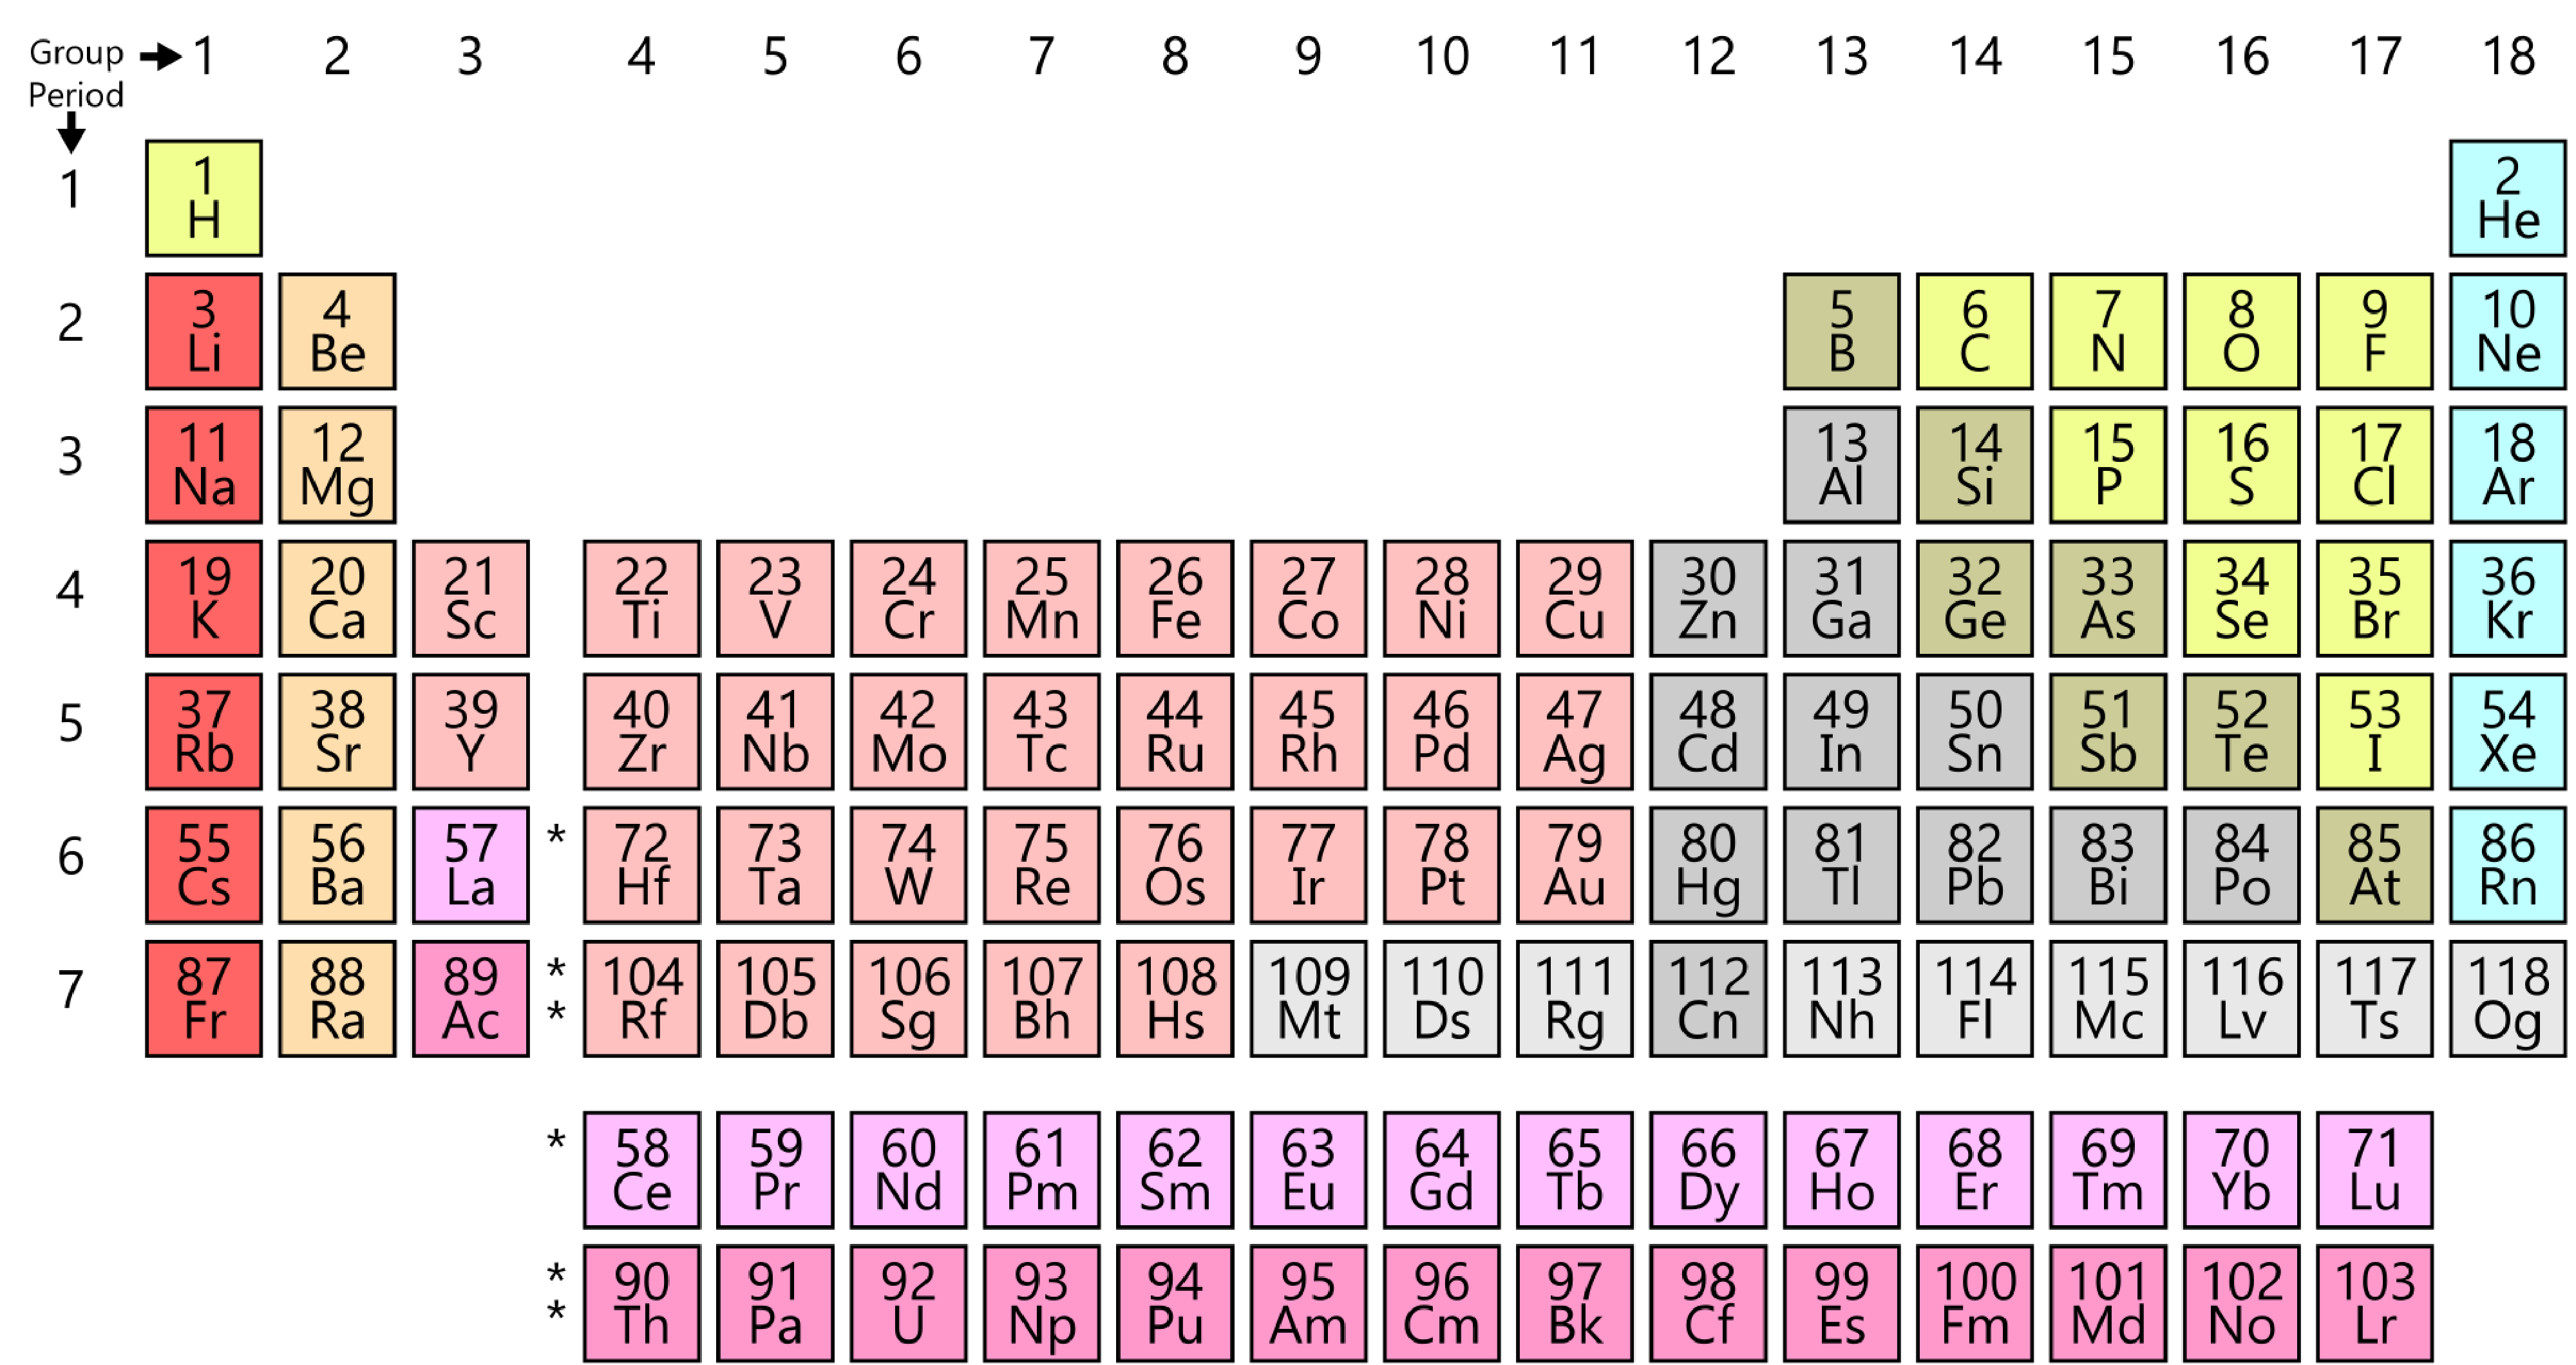
\includegraphics[width=.5\columnwidth]{periodic_table}
\end{center}
\caption{X. } \label{fig:periodic_table}
\end{figure}

Have a look at the periodic table reproduced here in Fig.~\ref{fig:periodic_table}.  You may recognize that many semicondutors are either Group III, IV, or V elements.   What's special about Group III, IV, and V elements?  Recall that the number of outer shell electrons in atoms is related to its group number.  Noble gases are unique in that they have complete shells and this is in fact why they are so stable.  Group IV elements in particular have four electrons in their out shell.  This is why when they are grouped together, they bond and share electrons, four electrons on average.


\subsection{Electronic Properties of Silicon}
  
We'll focus on silicon, but a lot of what we have to say applies to most semiconductors.  Silicon is the most commonly used semiconductor, so it's the most relevant example.  From chemistry, we know that silicon is in Group IV element, like carbon.  It has the following structure shown in Fig.~\ref{fig:slide20}:
  
\begin{itemize}
\item    Atom electronic structure: 1s$^2$2s$^2$2p$^6$3s$^2$3p$^2$
\item   Crystal electronic structure: 1s$^2$2s$^2$2p$^6$3(sp)$^4$
\item    Diamond lattice, with 0.235 nm bond length
\end{itemize}
   
Notice that the s and p orbitals combine when the silicon atoms combine into a hybridized state.  This deserves a bit of explanation.  When silicon atoms are far apart, the electrons occupy the usual orbital states you're familiar with from chemistry.  But when the atoms are brought into close proximity, the outer shell valence electrons feel the influence of two nuclei, and therefore it's logical to assume that the electrons should spend more time in between the nuclei, essentially forming covalent bonds.  If the Pauli exclusion principle didn't apply, then all the electrons would occupy the p orbitals in between the silicon atoms, leaving some empty and some more than full !  But alas only 2 electrons per orbital (with opposite spin).

On the other hand, the geometry of the p orbitals shown in Fig.~\ref{fig:slide20} would be ideal if silicon could bond to six neighbors, but there aren't enough electrons to go around since silicon only needs 4 additional electrons to form a complete shell.  On the other hand, the hybridized 3(sp)$^4$ state (linear combination of s and p orbitals) contains four electrons and can bond with four neighbors as shown.  This scenario is how silicon atoms combine to form a crystal, with the geometry more complicated than a simple cube  arising from these bond angles.


Also, silicon is a very poor conductor at room temperature. Why?
 
\begin{figure}
\begin{center}
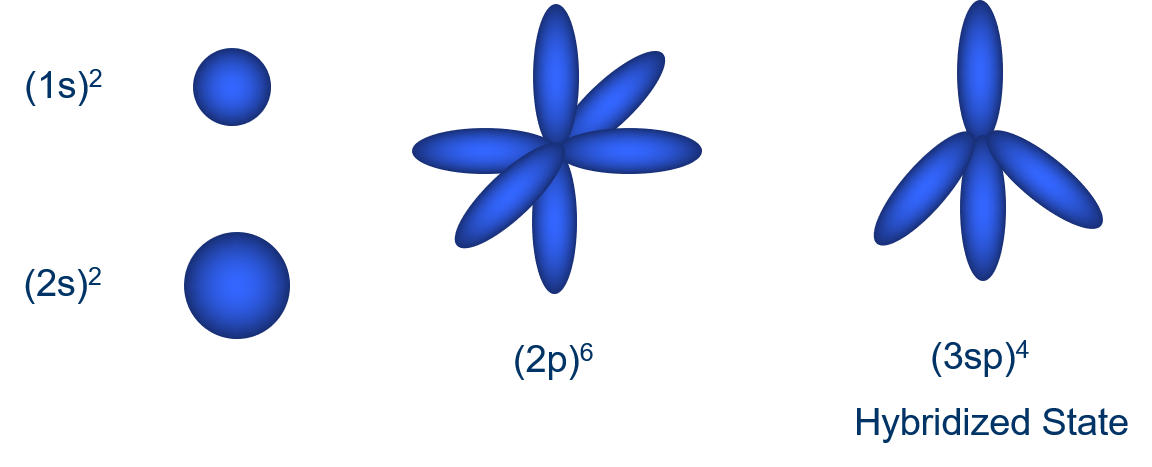
\includegraphics[width=.5\columnwidth]{slide20}
\end{center}
\caption{slide 20 structure of sli. } \label{fig:slide20}
\end{figure}

\subsubsection{Si Diamond Structure}


\begin{figure}
\begin{center}
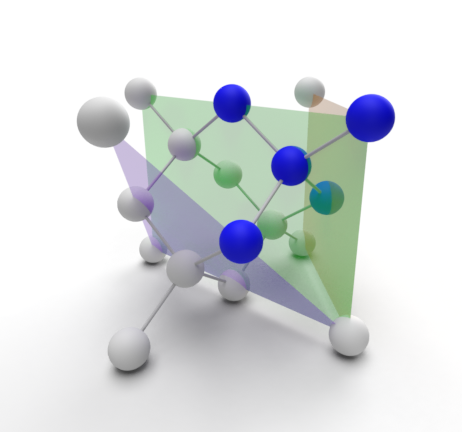
\includegraphics[width=.5\columnwidth]{silicon_crysal.png}
\end{center}
\caption{X. } \label{fig:silicon_crysal}
\end{figure}

Silicon atoms arrange in a nice crystal structure known as the diamond structure shown in Fig.~\ref{fig:silicon_crysal}.  In this figure, spheres represent silicon atoms with one particular unit cell highlighted.  The planes in the figure correspond to the symmetry planes of the crystal.  Usually the crystal is cut along one of these symmetry planes.

Notice that each silicon atom bonds to four neighbors using a covalent (shared electron) bond.  In a covalent bonds, the electrons are shared among a group of host atoms, giving up their identity and loyalty to a fixed atom as they are shared among a group of nuclei, forming a more stable overall structure than if they remained in their lone atomic orbitals.  The inner core electrons, on the other hand, are bound to the host nucleus and don't participate in conduction (the interest of this chapter) unless very energetic particles such as x-rays are incident on the crystal.  



\subsection{States of an Atom}

\begin{figure}
\begin{center}
\includegraphics[width=.5\columnwidth]{slide23}
\end{center}
\caption{X. } \label{fig:slide23}
\end{figure}


From quantum mechanics and chemistry,  we know that for an atom the allowed energy levels for an atom are discrete (2 electrons can occupy a state since with opposite spin), as shown in Fig.~\ref{fig:slide23}a.  There is an energy gap between states that electrons cannot occupy.   From solid-state physics, we have an important result that when a collection of atoms are brought together, the energy levels split as shown in Fig.~\ref{fig:slide23}b.   If there are a large number of atoms, the discrete energy levels form a nearly “continuous” band.   The gap between the energy levels may widen or even disappear, giving rise to different material properties.
 

\subsection{Energy Band Diagram}

In the energy diagram discussed, the lines represent allowed energy levels and the gaps represent levels that are simply not supported, they are forbidden.  This arises from the wave properties of the electron.  When an electron "orbits" an atom, we know that its orbit corresponds to the an integer number of de Broglie wavelengths.  In essence, when in such orbits, the electron wave experiences constructive interference whereas in other orbits it experiences destructive interference.  Because the square magnitude of the "wave" is the probability to find the electron, we find it's more probable for electrons to occupy these orbits.  This is a very simple perspective, but it got people like Niels Bohr to plunge ahead and develop a model for an atom.   In a collection of "free" electrons confined to the crystal "box", the spatial confinement results in a discrete energy (and momentum) spectrum.  The allowed energy levels are essentially a result of the boundary condition that requires that electrons are confined to the box with effectively zero probability to appear outside of the box.  When boundary conditions are imposed on the wave function, a discrete spectrum of allowed states results.  

In a similar way, for a collection of atoms, the forbidden energy states cannot be occupied by electrons.    Lower energy states correspond to "valence band" electrons, or electrons that are bound to host atoms.  Higher energy states, in the "conduction band" are "free" electrons that take part in conduction, as they are free to move around the crystal.  In essence, the conduction band electrons have sufficient energy to leave the nucleus and roam the crystal.  The host atoms become ionized and charged as a result.   The electrons act like free electrons in a vacuum, albeit with a different mass.\footnote{The electrons are still bound to reside in the crystal, and a significant amount of energy is required to remove these electrons from the crystal due to the fact that the entire crystal is charge neutral and leaving the crystal means charge separation}.  

The gap between the conduction and valence band determines the conductive properties of the material, see Fig.~\ref{fig:slide24b}.  In insulators, the gap between the conduction band and  valence band, or the band gap, is quite large,  $\sim 4-8$eV.  Therefore it takes an enormous amount of energy to pull electrons away from host atoms.  At room temperature, electrons only have an energy of about 25meV, so an $4$eV band gap is nearly an infinite one to overcome.  

In a metal, the conduction band is partially filled and therefore many electrons are free to move about, resulting in good conduction properties.  The band gap is either very small, or partially overlapping with the valence band, resulting in no discernible bandgap.  And this leaves semiconductors, which are materials that have a "medium sized" gap, about $\sim 1$eV.  This means that the barrier to become a free electron is high, but not impossible.  In a given solid of semiconductor, there's alawys a few lucky electrons that will be in the conduction band.  In fact, the probability of occupying  a certain energy level is related to the Boltzmann distribution modified to account for the fact that electrons are Fermions and cannot occupy the same energy levels, resulting in Fermi-Dirac statistics.


\begin{figure}
\begin{center}
\includegraphics[width=.5\columnwidth]{slide24b}
\end{center}
\caption{X. } \label{fig:slide24b}
\end{figure}

As discussed previously, thermal energy is very low on average ($\sim 25$meV), but there are a few (very few) high energy electrons.   So the conductivity of semiconductors is poor, but not zero.  As shown in Fig.~\ref{fig:slide24}, electrons in the valence band can gain energy from incoming photons or from the vibration in the crystal (phonons) and if the energy is sufficiently large, they can absorb  it and go into the conduction band.


\begin{figure}
\begin{center}
\includegraphics[width=.5\columnwidth]{slide24}
\end{center}
\caption{X. } \label{fig:slide24}
\end{figure}


\subsection{Model for Good Conductor}
  
Given this background, we can now model a good conductor as a collection of atoms that are all ionized forming a  “sea” of electrons can wander about crystal, shown in Fig.~\ref{fig:slide25}.   The electrons are the “glue” that holds the solid together.  They spend most of their time in between the ionized nuclei, effectively shielding the nuclei from each other, lowering the energy of the system.  But they are not confined to bonds, they are free to move around the crystal and contribute to conduction.  Since they are “free”, they respond to applied fields and give rise to ohmic currents.  They also respond to incoming photons and give rise to the optical properties such as the fact that these materials are opaque and have shiny surfaces.   Electrons at the surface of the structure readily accept optical photons and re-radiate them.
 


\begin{figure}
\begin{center}
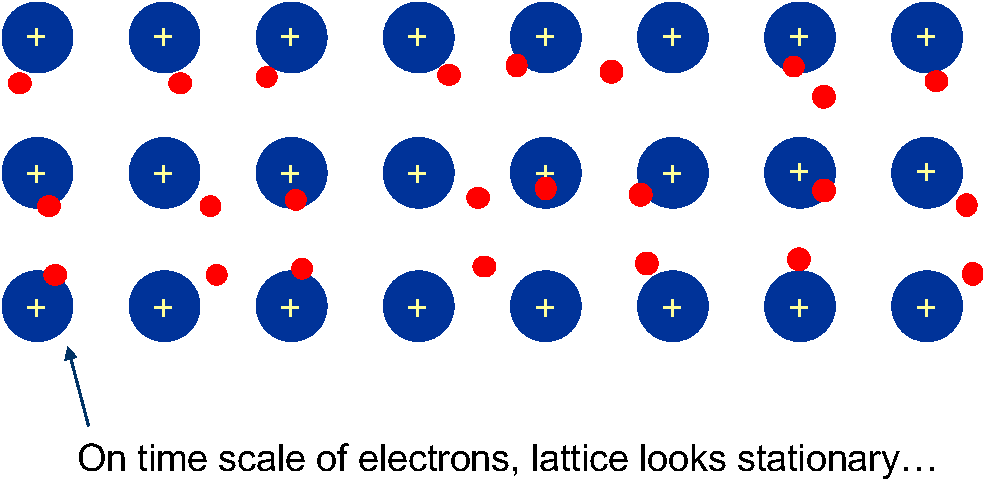
\includegraphics[width=.5\columnwidth]{slide25}
\end{center}
\caption{Model for good conductor. } \label{fig:slide25}
\end{figure}

 





\subsubsection{Semiconductor Bond Model}

Unlike a conductor, a semiconductor does not have many free electrons.  This is because all of the electrons are forming bonds in the crystal.  How can we free electrons ?  Either by giving them enough energy to break free (photons or very high energy phonons) or we have to introduce impurities in the crystal structure that have a different number of bonding electrons.  We'll discuss this in details next.

\subsection{Bond Model for Silicon ($T=0$K)}

Let's build a simple 2D model for silicon as shown in Fig.~\ref{fig:silicon_model}.  The circles represent the nuclei and the lines represent electrons that are forming covalent bonds, or residing in the 3(sp)$^4$ orbitals.  For simplicity, we squashed the orbitals to lie on a plane.

\begin{figure}
\begin{center}
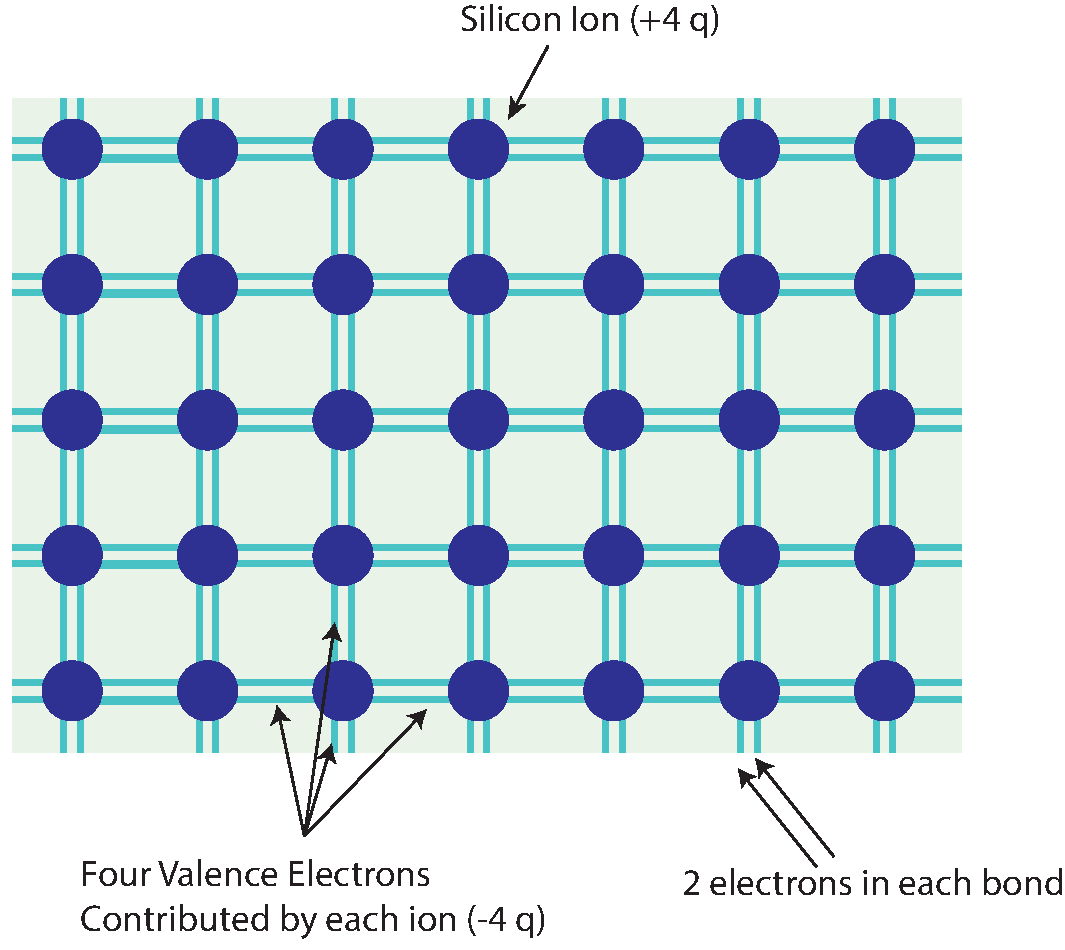
\includegraphics[width=.5\columnwidth]{silicon_model}
\end{center}
\caption{Model for silicon at $T=0^\circ$K. } \label{fig:silicon_model}
\end{figure}

Each bond holds two electrons with opposite spin.  Each atom contributes 4 valence electrons to the orbital and borrows 4 electrons from 4 neighbors.  Thus each atom experiences a lower energy state corresponding to having a full orbital, despite being a group 4 element.  All the electrons are busy orbiting the nuclei and none can contribute to current conduction.


\subsection{Bond Model for Silicon ($T>0$K)}

\begin{figure}
\begin{center}
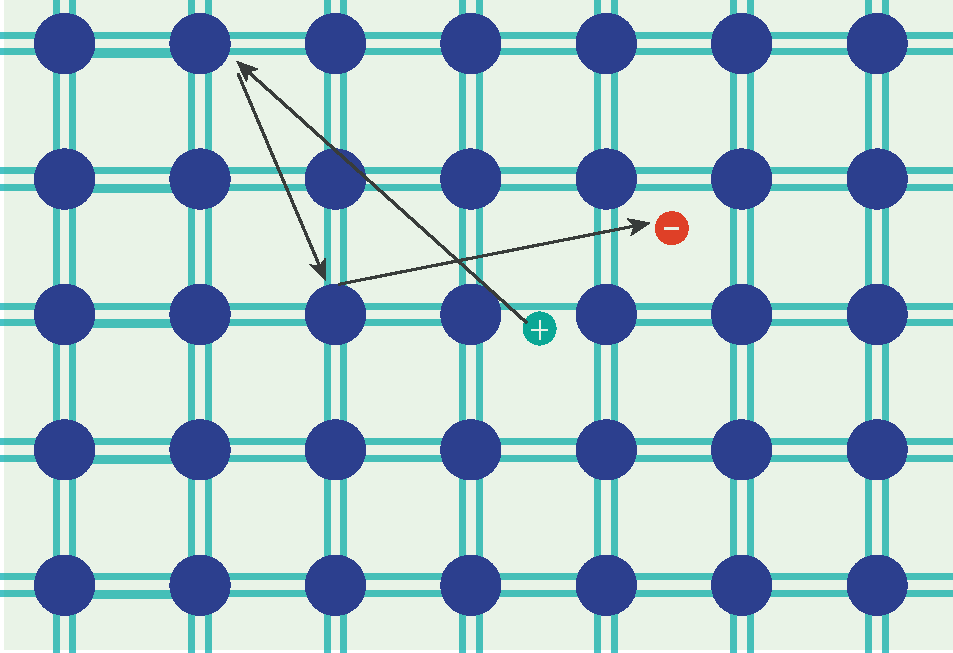
\includegraphics[width=.5\columnwidth]{silicon_broken_bond}
\end{center}
\caption{X. } \label{fig:silicon_broken_bond}
\end{figure}

Now let's suppose we increase the temperature, which means the crystal lattice can absorb energy in the form of vibrations.  Quantum mechanically, these vibrations can be treated as particle "phonons" (in analogy with photons) which can exchange energy with the electrons.  Occasionally enough energy can be absorbed by a valence electron to be broken free from the lattice structure.  In the energy band model, we know the energy absorbed has to be at least as large as the band gap.  Once an electron becomes a conduction band electron, it's free.  It can roam the crystal like a free electron.  The mass of the electron is not the same as the mass of an electron in a pure vacuum.  That's because the electron will still feel the influence of the crystal potential, which varies periodically.  It turns out that we can define an "effective" mass for the electron and treat it as if it were free and in vacuum, free from the influence of the crystal potential.  


\subsection{Holes?}

When we formed a free electron, we leave behind a broken bond.  This bond means the host atom has net charge.  But this charge corresponding to the vacancy is "fixed", right?

\begin{figure}
\begin{center}
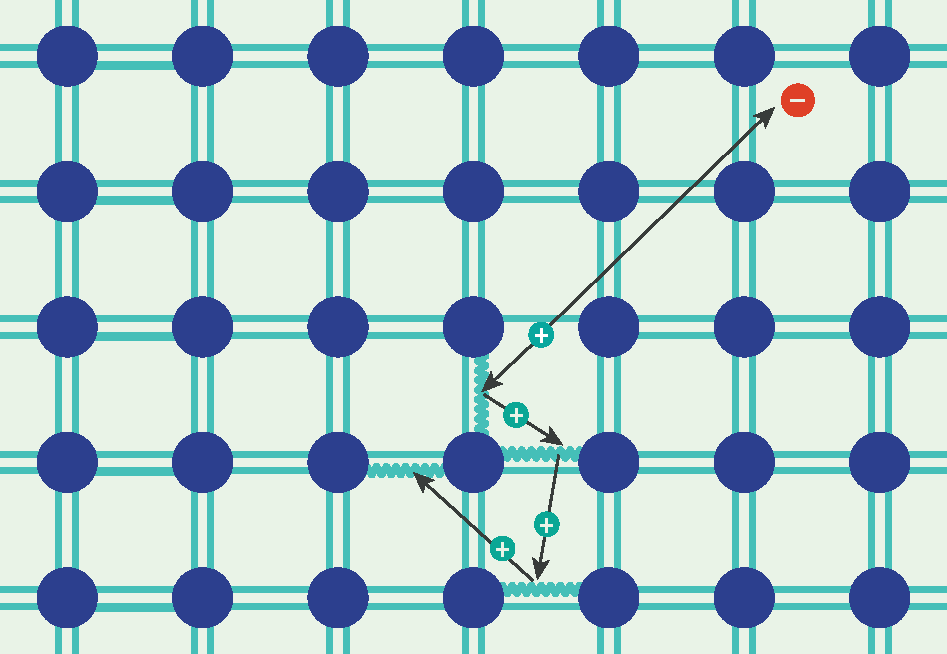
\includegraphics[width=.5\columnwidth]{silicon_hole}
\end{center}
\caption{X. } \label{fig:silicon_hole}
\end{figure}
  
Notice that the vacancy (hole) left behind can be filled by a neighboring electron.   But if the neighboring electron jumps into this vacancy, it forms it's own vacancy while filling the other one.  This chain reaction of vacancies moving around is complex as it corresponds to the motion of many valence band electrons.  An easy way to model it is to great it like there is a positive charge traveling around.  We call this positive (ficticious) particle a "hole".  We can treat the holes as legitimate particles with mass and charge.
 


\subsection{Yes, Holes!}

The net motion of many electrons in the valence band can be equivalently represented as the motion of a hole.  The picture is more complicated because electrons near the valence band edge have negative effective mass !  This is why the hole model is works as it does.  
 

\begin{equation}
{J_{vb}} = \sum\limits_{vb} {( - q){v_i}}  = \sum\limits_{Filled\,Band} {( - q){v_i} - \sum\limits_{Empty\,States} {( - q){v_i}} } 
\end{equation}

\begin{equation}
{J_{vb}} =  - \sum\limits_{Empty\,States} {( - q){v_i}}  = \sum\limits_{Empty\,States} {q{v_i}} 
\end{equation}





\subsection{More About Holes}


  
 When a conduction band electron encounters a hole, the process is called \textit{recombination}
 The electron and hole annihilate one another thus depleting the supply of carriers
 In thermal equilibrium, a generation process counterbalances to produce a steady stream of carriers
 






\section{Intrinsic Carrier Concentration}











\subsection{Thermal Equilibrium (Pure Si)}


  
 Balance between generation and recombination determines $n_0 =  p_0 $
 Strong function of temperature:  $T = 300^\circ$K
 


\begin{equation} G = {G_{th}}(T) + {G_{opt}} \end{equation}
\begin{equation} R = k(n \times p) \end{equation}
\begin{equation} G = R \end{equation}
\begin{equation} k(n \times p) = {G_{th}}(T) \end{equation}
\begin{equation} n \times p = {G_{th}}(T)/k = {n_i}^2(T) \end{equation}
\begin{equation} {n_i}(T) \cong {10^{10}}{\rm{c}}{{\rm{m}}^{ - 3}}\,{\rm{at}}\,300\,{\rm{K}}
\end{equation}





\subsection{Generation Statistics}


  
 The rate at which carriers are generated is a strong function of the material bandgap $E_g$ (the distance between the valence band and conduction band), because it takes that much energy to promote an electron [or that much energy to break the bond]
 Since the mechanism for is \textit{thermal} (vibrations), the hotter the temperature, the more generation
 It can be shown that the rate of generation is given by the following equation:

\begin{equation}
	n_i \propto e^{-E_g/2kT}
\end{equation}
 






\section{Doping with Impurities}










\subsection{Doping with Group V Elements}

 P, As (group 5): extra bonding electron … lost to crystal at room temperature



\begin{figure}
\begin{center}
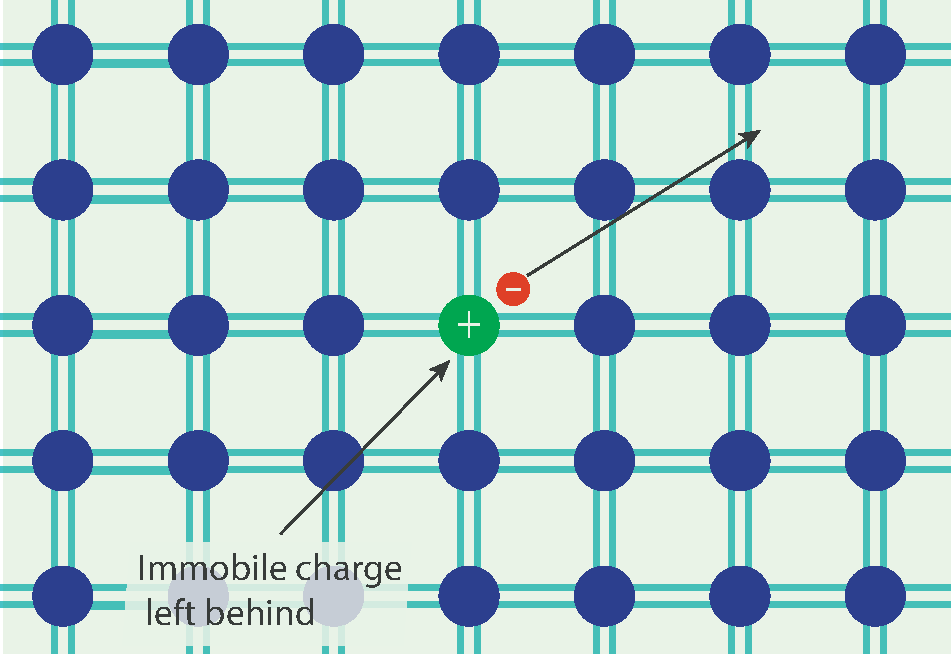
\includegraphics[width=.5\columnwidth]{silicon_dopant_V}
\end{center}
\caption{X. } \label{fig:silicon_dopant_V}
\end{figure}




\subsection{Donor Accounting}

 Each ionized donor will contribute an extra “free” electron

 The material is charge neutral, so the total charge concentration must sum to zero:


\begin{equation}
	\rho  =  \underbrace{- q{n_0}}_{\text{free electrons}} 
	+ \underbrace{q{p_0}}_{\text{free holes}} + 
	\underbrace{q{N_d}}_{\text{ions (immobile)}}  = 0
\end{equation}


 By Mass-Action Law:  $n \times p = {n_i}^2(T)$
\begin{equation}
	 - q{n_0} + q\frac{{n_i^2}}{{{n_0}}} + q{N_d} = 0
\end{equation}
\begin{equation}
 - qn_0^2 + qn_i^2 + q{N_d}{n_0} = 0
\end{equation}






\subsection{Donor Accounting (cont)}


  
 Solve quadratic:  $n_0^2 - {N_d}{n_0} - n_i^2 = 0$

\begin{equation}
	{n_0} = \frac{{{N_d} \pm \sqrt {N_d^2 + 4n_i^2} }}{2}
\end{equation}
 Only positive root is physically valid:

\begin{equation}
	{n_0} = \frac{{{N_d} + \sqrt {N_d^2 + 4n_i^2} }}{2}
\end{equation}
 For most practical situations:  ${N_d} \gg {n_i}$
\begin{equation}
{n_0} = \frac{{{N_d} + {N_d}\sqrt {1 + 4{{\left( {\frac{{{n_i}}}{N}} \right)}^2}} }}{2} \approx \frac{{{N_d}}}{2} + \frac{{{N_d}}}{2} = {N_d}
\end{equation}
 





\subsection{Doping with Group III Elements}

 Boron: 3 bonding electrons $\rightarrow$ one bond is unsaturated
 Only free hole … negative ion is immobile!
 

\begin{figure}
\begin{center}
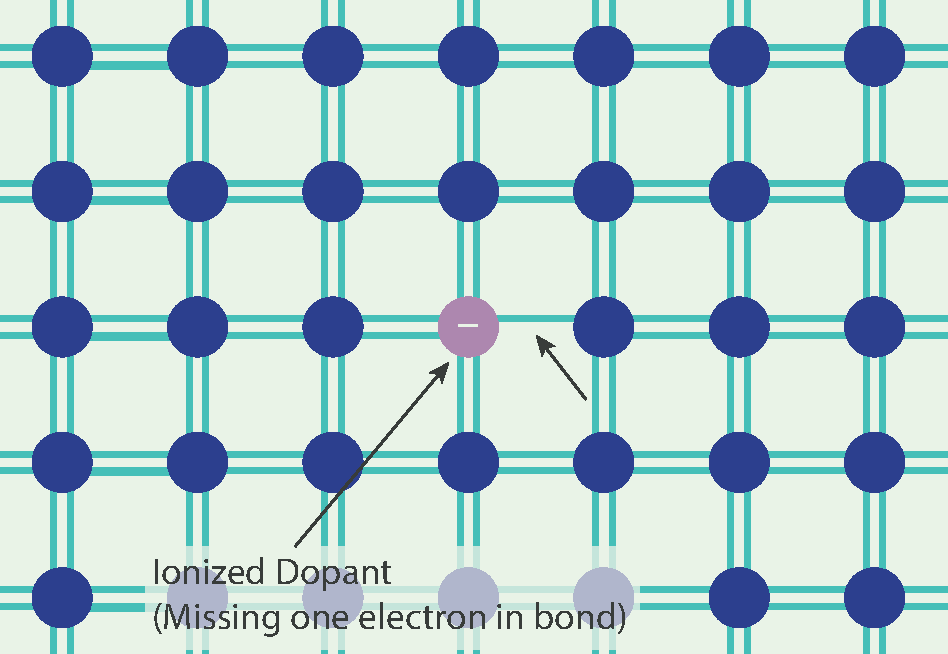
\includegraphics[width=.5\columnwidth]{silicon_dopant_III}
\end{center}
\caption{X. } \label{fig:silicon_dopant_III}
\end{figure}




\subsection{Mass Action Law}  
 Balance between generation and recombination:  
\begin{equation}
	{p_o} \cdot {n_o} = {n_i}^2
\end{equation}  
($(T = 300\,{\rm{K}},\,\,{n_i} = {10^{10}}{\rm{c}}{{\rm{m}}^{ - 3}})$)
 { N-type case: }  ${n_0} = N_d^ +  \cong {N_d}$
\begin{equation}
	p_0 = \frac{n_i^2}{N_d}
\end{equation}
 { P-type case:}  ${p_0} = N_a^ -  \cong {N_a}$  
\begin{equation}
	n_0 = \frac{n_i^2}{N_a}
\end{equation}

 




\subsection{Compensation}


 Dope with \textit{both} donors and acceptors:
  
    Create free electron and hole!
 




\begin{figure}
\begin{center}
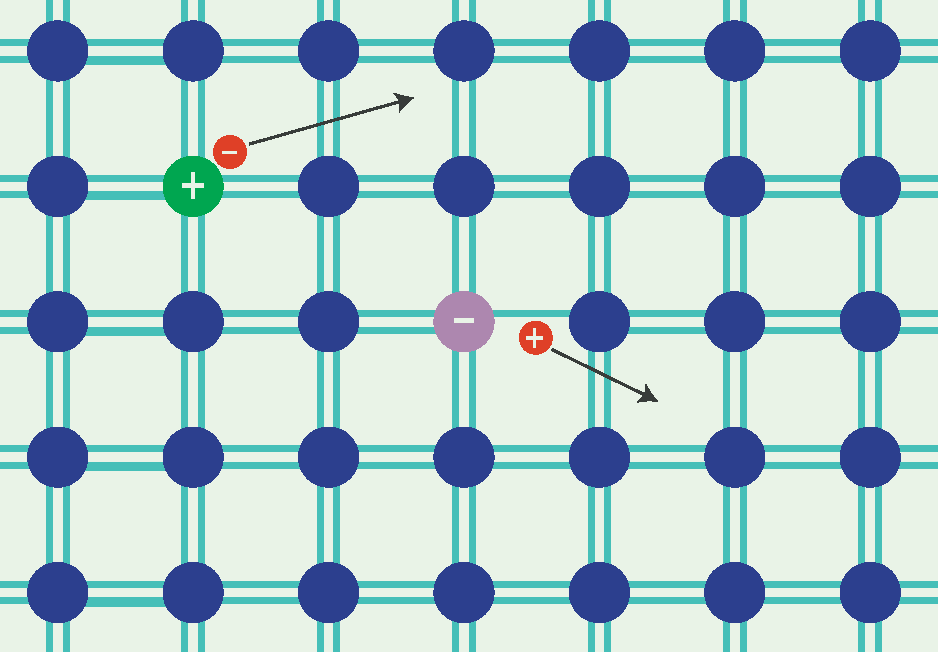
\includegraphics[width=.5\columnwidth]{silicon_dopant_both}
\end{center}
\caption{X. } \label{fig:silicon_dopant_both}
\end{figure}




\subsection{Compensation (cont.)}


 More donors than acceptors:   $N_d > N_a$


\begin{equation}
	{n_o} = {N_d} - {N_a} \gg {n_i}
\end{equation}


\begin{equation}
	{p_o} = \frac{{n_{_i}^2}}{{{N_d} - {N_a}}}
\end{equation}

 More acceptors than donors:  $N_a > N_d$


\begin{equation}
	{n_o} = {N_a} - {N_d} \gg {n_i}
\end{equation}


\begin{equation}
	{n_o} = \frac{{n_{_i}^2}}{{{N_a} - {N_d}}}
\end{equation}








\section{Drift Currents}











\subsection{Thermal Equilibrium}


 Rapid, random motion of holes and electrons at “thermal velocity” $v_{th} = 10^7$ cm/s with collisions every $\tau_c = 10^{-13}$s.
\begin{equation}
	{\textstyle{1 \over 2}}m_n^*v_{th}^2 = {\textstyle{1 \over 2}}kT
\end{equation}
 Apply an electric field $E$ and charge carriers accelerate … for $\tau_c$ seconds






\begin{figure}
\begin{center}
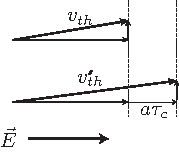
\includegraphics[width=.5\columnwidth]{drift_field}
\end{center}
\caption{X. } \label{fig:drift_field}
\end{figure}
\begin{equation} \lambda  = {v_{th}}{\tau _c}\end{equation}
\begin{equation} 
	\lambda  = {10^7}{\rm{cm}}/s \times {10^{ - 13}}s = {10^{ - 6}}{\rm{cm}}
\end{equation}
(hole case)





\subsection{Drift Velocity and Mobility}

 For holes:   ${v_{dr}} = {\mu _p}E$

\begin{equation} 
	{v_{dr}} = a \cdot {\tau _c} = \left( {\frac{{{F_e}}}{{{m_p}}}} \right){\tau _c} = \left( {\frac{{qE}}{{{m_p}}}} \right){\tau _c} = \left( {\frac{{q{\tau _c}}}{{{m_p}}}} \right)E
\end{equation}
 For electrons:  ${v_{dr}} = -{\mu _n}E$

\begin{equation} 
	{v_{dr}} = a \cdot {\tau _c} = \left( {\frac{{{F_e}}}{{{m_n}}}} \right){\tau _c} = \left( {\frac{{-qE}}{{{m_n}}}} \right){\tau _c} = -\left( {\frac{{q{\tau _c}}}{{{m_n}}}} \right)E
\end{equation}






\subsection{Mobility vs. Doping in Silicon at $300^\circ$K}
\begin{center}

\begin{figure}
\begin{center}
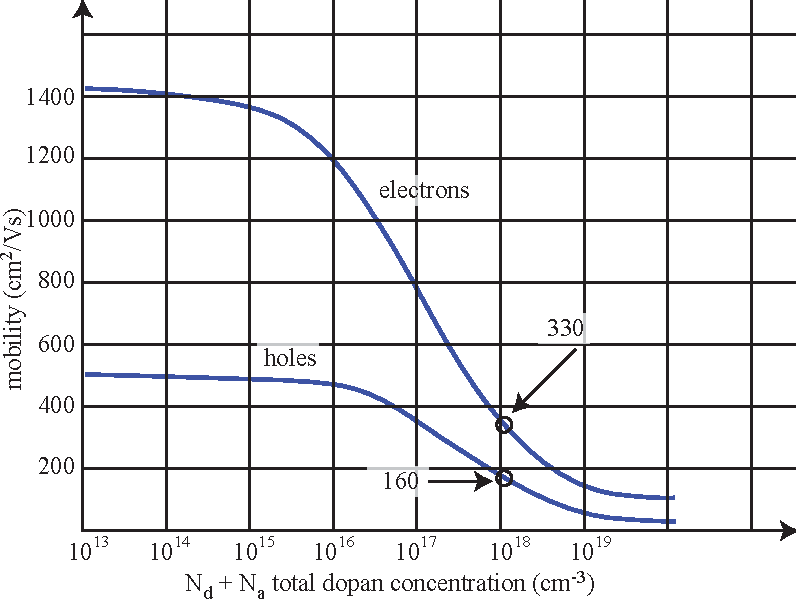
\includegraphics[width=.5\columnwidth]{mobility}
\end{center}
\caption{X. } \label{fig:mobility}
\end{figure}
\end{center}


 Typical values: ${\mu _n} = 1000 \mathrm{cm^2}/\mathrm{V s}$ and ${\mu _p} = 400 \mathrm{cm^2}/\mathrm{V s}$.






\section{Diffusion Currents}











\subsection{Diffusion}
  
 Diffusion occurs when there exists a concentration gradient
 In the figure below, imagine that we fill the left chamber with a gas at temperate $T$
 If we suddenly remove the divider, what happens?
 The gas will fill the entire volume of the new chamber. How does this occur?
 





\begin{figure}
\begin{center}
\includegraphics[width=.5\columnwidth]{slide46}
\end{center}
\caption{X. } \label{fig:slide46}
\end{figure}

\begin{figure}
\begin{center}
\includegraphics[width=.5\columnwidth]{slide46b}
\end{center}
\caption{X. } \label{fig:slide46b}
\end{figure}




\subsection{Diffusion (cont)}

\begin{figure}
\begin{center}
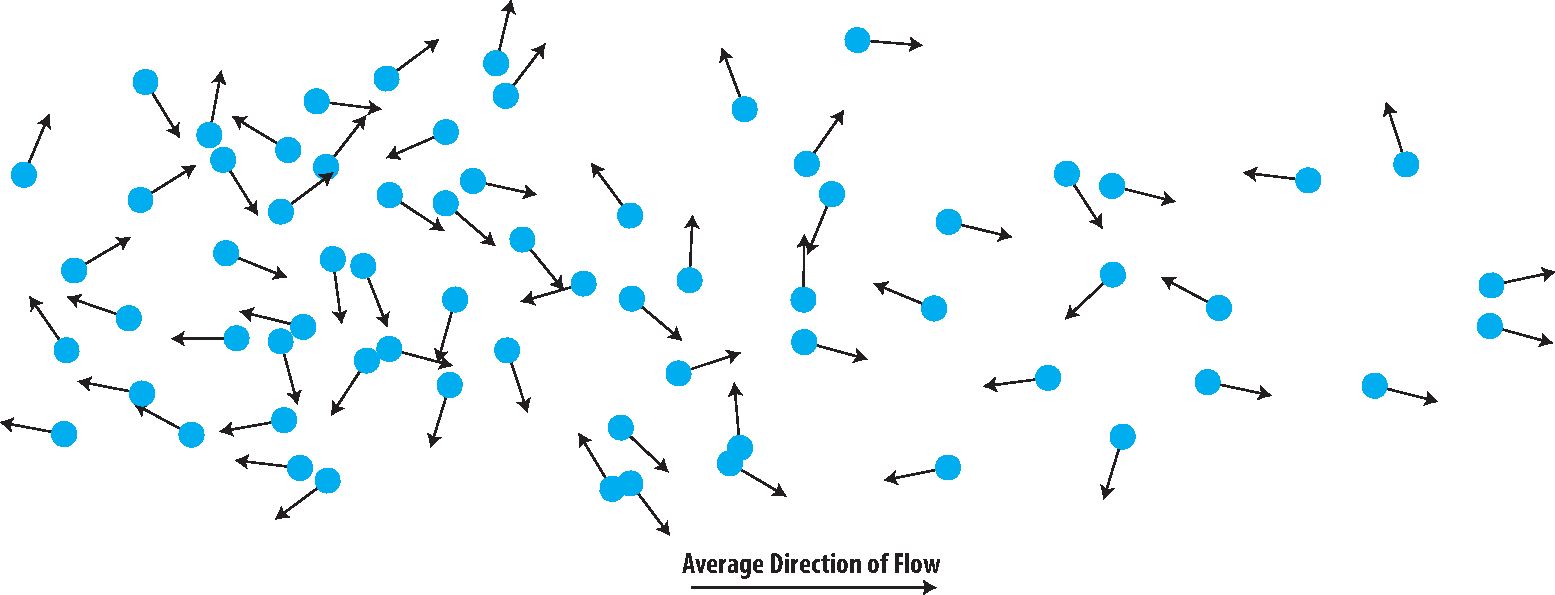
\includegraphics[width=.5\columnwidth]{random_flow}
\end{center}
\caption{X. } \label{fig:random_flow}
\end{figure}

  
 The net motion of gas molecules to the right chamber was due to the concentration gradient
 If each particle moves on average left or right then eventually half will be in the right chamber. If the molecules were charged (or electrons), then there would be a net current flow.
 It's clear that the diffusion current flows from high concentration to low concentration.
 





\subsection{Diffusion Equations}
  
 Assume that the mean free path is $\lambda$
 Find flux of carriers crossing $x=0$ plane
 



\begin{figure}
\begin{center}
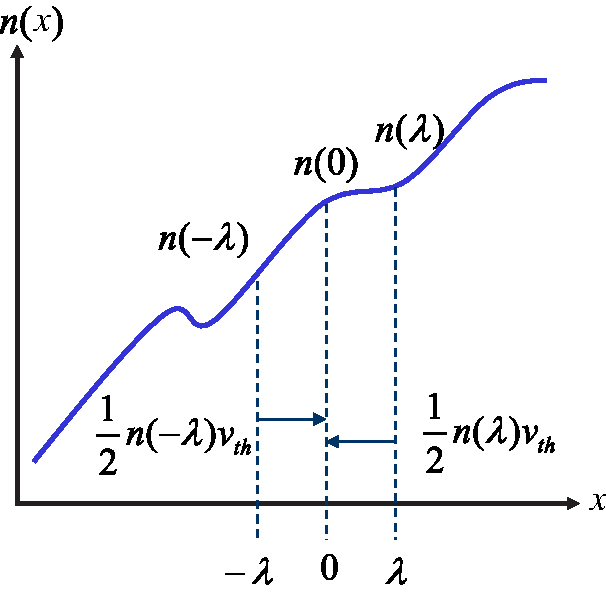
\includegraphics[width=.5\columnwidth]{slide48}
\end{center}
\caption{X. } \label{fig:slide48}
\end{figure}

\begin{equation}
	F = \frac{1}{2}{v_{th}}\left( {n( - \lambda ) - n(\lambda )} \right)
\end{equation}
\begin{equation}
	F = \frac{1}{2}{v_{th}}\left( {\left[ {n(0) - \lambda \frac{{dn}}{{dx}}} \right] -
	 \left[ {n(0) + \lambda \frac{{dn}}{{dx}}} \right]} \right)
\end{equation}
\begin{equation}
	F =  - {v_{th}}\lambda \frac{{dn}}{{dx}}
\end{equation}
\begin{equation}
	J =  - qF = q{v_{th}}\lambda \frac{{dn}}{{dx}}
\end{equation}






\subsection{Einstein Relation}
  
 The thermal velocity is given by $T$
 

\begin{equation}
	{\textstyle{1 \over 2}}m_n^*v_{th}^2 = {\textstyle{1 \over 2}}kT
\end{equation}
Mean Free Path / Time:
\begin{equation}
	\lambda  = {v_{th}}{\tau _c}
\end{equation} 
\begin{equation} 
	{v_{th}}\lambda  = v_{th}^2{\tau _c} = kT\frac{{{\tau _c}}}{{m_n^*}} = \frac{{kT}}{q}\frac{{q{\tau _c}}}{{m_n^*}}
\end{equation}
\begin{equation}
	J = q{v_{th}}\lambda \frac{{dn}}{{dx}} = q\left( {\frac{{kT}}{q}{\mu _n}} \right)\frac{{dn}}{{dx}}
\end{equation}
\begin{equation}
	{D_n} = \left( {\frac{{kT}}{q}} \right){\mu _n}
\end{equation}





\subsection{Total Current and Boundary Conditions}
  
 When both drift and diffusion are present, the total current is given by the sum:
\begin{equation}
	J = {J_{drift}} + {J_{diff}} = q{\mu _n}nE + q{D_n}\frac{{dn}}{{dx}}
\end{equation}
 In resistors, the carrier is approximately uniform and the second term is nearly zero
 For currents flowing uniformly through an interface (no charge accumulation), the field is discontinuous:
 



\begin{figure}
\begin{center}
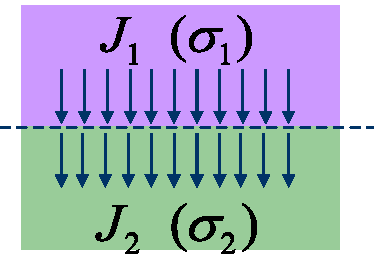
\includegraphics[width=.5\columnwidth]{slide50}
\end{center}
\caption{X. } \label{fig:slide50}
\end{figure}
\begin{equation} {J_1} = {J_2}\end{equation}
\begin{equation}{\sigma _1}{E_1} = {\sigma _2}{E_2}\end{equation}
\begin{equation}\frac{{{E_1}}}{{{E_2}}} = \frac{{{\sigma _2}}}{{{\sigma _1}}}\end{equation}





\subsection{Reference}


  
 Edward Purcell, \textit{Electricity and Magnetism}, Berkeley Physics Course Volume 2 (2nd Edition), pages 133-142.
 



